\chapter[Introdução]{Introdução} \label{cap:introducao}
% \addcontentsline{toc}{chapter}{Introdução}

A democracia digital é resumida por \citeonline{penteadoencontro} como o uso da Internet para consolidação da democracia.
Este uso tem acarretado um crescente número de discussões acerca de temas políticos, o que permitiu que interessados na área analisassem esse fenômeno e observassem uma 
polarização das mensagens trocadas nas redes sociais \cite{empurrandojuntos}.

\citeonline{empurrandojuntos} afirmaram que as discussões realizadas, principalmente em redes sociais, 
acabavam refletindo sempre a opinião da maioria e que as pessoas estão sempre presentes em uma bolha de opinião. 
Isto é, os algoritmos dessas plataformas selecionam o conteúdo a ser apresentado de acordo com o comportamento anterior,
no qual foi coletada a opinião deste usuário.
Dessa forma, essa polarização dificulta a explanação das ideias da minoria e restringe a apresentação de pensamentos diferentes para quem usa essas redes sociais. 

Observando esse aspecto, o Instituto Cidade Democrática\footnote{Site do Cidade Democrática: \url{http://www.cidadedemocratica.org.br/}} 
apresenta a plataforma ``Empurrando Juntos'' cujo objetivo 
é dar voz para a minoria e tornar as discussões mais efetivas para os seus propósitos \cite{empurrandojuntos}.

A ideia é que um usuário entre em um \textit{website} ou em um aplicativo de celular para criar conversas e 
participar de conversas criadas por outros usuários. Essa participação 
acontece de duas formas: comentando uma conversa ou votando em um comentário de outro participante. Entende-se por voto
o ato de concordar com o comentário realizado (uma espécie de \textit{like}) ou discordar do comentário. Além disso, é permitido
que o usuário pule aquele comentário, ou seja, não atribua nenhum tipo de voto \cite{empurrandojuntos}. 

Com os votos realizados, é possível agrupar pessoas que responderam de maneira parecida, ou seja, concordaram e
discordaram dos mesmos comentários. Com os grupos formados, é possível ver a convergência e divergência de opiniões, 
prover ao usuário uma visão ampliada das opiniões acerca do assunto e promover a interação entre os usuários com 
pensamentos divergentes. A Figura \ref{fig:resumo_ej} ilustra o funcionamento completo do sistema.


\begin{figure}[h!]
\centering
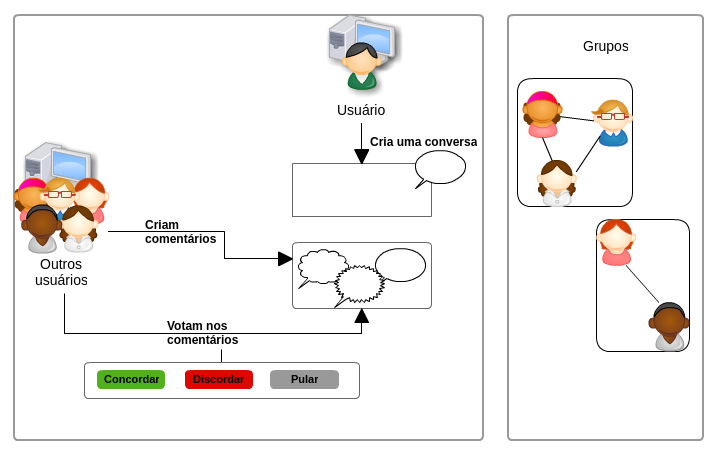
\includegraphics[scale=0.6]{figuras/resumo_ej.png}
\caption{Funcionamento do ``Empurrando Juntos''}
\label{fig:resumo_ej}
\end{figure}
% 
% Atualmente, o módulo que realiza a clusterização é a única funcionalidade em desenvolvimento na plataforma.
A parte de agrupamento é realizada em tempo real, ou seja, conforme as pessoas votam são formados ou modificados os grupos. 
Portanto, não há estabelecimento prévio dos grupos, são conhecidos apenas os dados em comum entre os usuários, que são os votos nas conversas. 
Sendo assim, nota-se a necessidade de um processo de classificação para que esses grupos sejam formados.

A partir do funcionamento estabelecido na Figura \ref{fig:resumo_ej} observa-se que o sistema pode ser dividido em dois processamentos: gestão de usuários 
e suas ações (criação de conversas, comentários e votos) e agrupamento destes usuários com base em seus votos.

Considerando esses aspectos, optou-se por uma arquitetura em três módulos: servidor, cliente e matemático. Na qual, o módulo servidor 
consiste em uma \textit{Application Programming Interface} (API), que de acordo com \citeonline{wagh2012comparative, understanding_web}
é uma interface que expõe os seus componentes como um serviço, permitindo que outras aplicações interajam com esses 
componentes. Desse modo, possibilita o compartilhamento dos dados armazenados com as aplicações que a consomem.

A parte cliente da aplicação é responsável pela interface visual do sistema e realiza a comunicação com a parte servidor no processamento
de usuários e ações no sistema. Por fim, o módulo matemático é responsável pela formação dos grupos de pessoas de acordo com os votos realizados.

% Com este agrupamento sendo realizado pela técnica de classificação.
% Trazer que existem tipos e inúmeras técnicas 


Considerando os aspectos supracitados, o objetivo do trabalho foi criar uma API para prover o gerenciamento dos usuários e conversas e a formação
dos grupos de pessoas para a plataforma ``Empurrando Juntos'', permitindo a utilização de diferentes
módulos matemáticos. 

Para realização do objetivo proposto, o trabalho foi dividido em cinco etapas, conforme a Figura \ref{fig:etapas_trabalho}. 

\begin{figure}[h!]
\centering
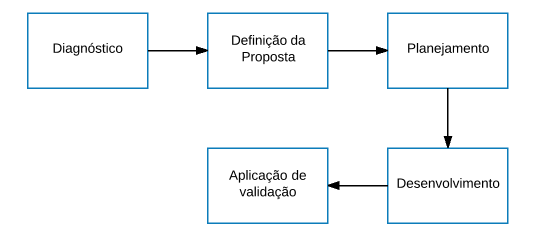
\includegraphics[scale=0.6]{figuras/etapas.png}
\caption{Etapas do trabalho}
\label{fig:etapas_trabalho}
\end{figure}

A etapa de ``Diagnóstico'' compreendeu o entendimento do escopo da plataforma ``Empurrando Juntos''. A etapa de ``Definição da Proposta'' foi caracterizada pela definição de escopo, 
da arquitetura da API e da comunicação com os módulos matemáticos. Na terceira etapa, foi feito o planejamento da execução do trabalho com o estabelecimento
de um cronograma com as atividades a serem realizadas nas próximas etapas. 

Na etapa de ``Desenvolvimento'' foram realizadas as iterações de implementação, teste e adaptação da API. Por fim, na etapa de ``Aplicação em um caso'' a API foi utilizada em uma 
plataforma de exemplo.

Nesse contexto, este trabalho, além desta introdução, está organizado em outros X capítulos. 
No Capítulo \ref{cap:api} são apresentados os conceitos e arquiteturas para APIs. O Capítulo \ref{cap:clusterizacao} aborda os conceitos e técnicas de 
classificação. A proposta do trabalho é apresentada no Capítulo \ref{cap:proposta} e por fim são apresentadas as conclusões no Capítulo 
\ref{cap:consideracoes_finais}.


% ############ VIOLENCIA CONTRA A MULHER #######################

% O propósito do ``Empurrando Juntos'' de incentivar esse tipo de discussão, com a exposição de todas as opiniões obtidas, é essencial para possibilitar mudanças neste âmbito político, 
% seja para promover debates sobre projetos de leis ou sobre outros assuntos de relevância, para criação de políticas públicas.

% Nesse contexto, uma das temáticas que tem se destacado nessas discussões é a de violência contra a mulher. Segundo \citeonline{violence_against_women}, 
% o termo violência contra a mulher trata de
% diversos atos de abuso e violência baseados no gênero, ou seja, dirigidos à mulheres e meninas ao longo da vida.
% De acordo com o estudo da \citeonline{violence_global}, dos diversos tipos de violência existentes, a violência doméstica, ou proveniente do parceiro,
% e a violência sexual, proveniente de um indivíduo diferente do parceiro, são as formas de violência que prevalecem.
% 
% \citeonline{violence_global}, em sua pesquisa, mostra que 
% 35\% das mulheres no mundo já vivenciaram 
% uma situação de violência física e/ou sexual pelo parceiro e violência sexual por outro indivíduo. No mundo, 38\% dos homicídios de mulheres são cometidos 
% pelos parceiros das vítimas.
% 
% No Brasil, de acordo com o Sistema de Informações sobre Mortalidade (SIM), entre 1980 e 2013, 106.093 mulheres foram vítimas de homicídio, 
% representando em 2013 uma taxa de aproximadamente 13 homicídios femininos
% diários \cite{mapa_violencia_2015}. 
% 
% Cenários como esses impulsionaram, além das discussões promovidas nas redes sociais, a criação de políticas públicas para a redução da violência 
% contra as mulheres e de estratégias de apoio às mulheres e de conscientização da população. Além disso, estratégias tecnológicas, 
% como aplicativos e sites, têm surgido nesse contexto.
% 
% No Brasil, a criação da Lei Maria da Penha, da Lei do Feminicídio e de programas e serviços de apoio à causa, 
% como o disque-denúncia Ligue 180, a Casa da Mulher Brasileira e a Unidade Móvel de Atendimento são respostas aos cenários supracitados. 
% No contexto de Tecnologia da Informação (TI), a criação de software têm sido apoiada pelo governo e realizada pela própria população.
% 
% Um levantamento que realizamos sobre as aplicações existentes no Brasil demonstra que a tecnologia é usada principalmente para: 
% prover uma rede de denúncias, para mapear locais de risco ou para levar essa denúncia até uma autoridade competente. Além disso, muitas aplicações 
% preocupam-se em prover informações sobre leis e conceitos.
% 
% Contudo, o cenário de violência contra a mulher no Brasil ainda deve ter atenção do governo e da sociedade. No primeiro semestre de 2016 
% foram contabilizados 555.634 atendimentos na central de denúncias 
% de violência contra a mulher, de acordo com o levantamento feito pela Secretaria de Políticas para as Mulheres (SPM). 
% Aproximadamente 54\% dos atendimentos foram para prestação de informações. De acordo com este levantamento \cite{portal_180}, aproximadamente 13\% dos 
% atendimentos, 
% são relatos de violência física (51\%), psicológica (31,1\%), moral (6,51\%), patrimonial (1,93\%), sexual (4,30\%), cárcere privado (4,86\%) e 
% tráfico de pessoas (0,24\%).
% 
% Observando esses aspectos, percebe-se que mesmo com as políticas e aplicações existentes, a promoção de discussões efetivas acerca do 
% assunto ainda é abaixo do esperado. Assim, nota-se a importância de promover essas discussões sobre a situação das mulheres a fim de 
% melhorá-la em diversos aspectos, seja criando uma rede de apoio entre as mulheres que enfrentam situações semelhantes ou chamando a atenção 
% para causas de interesse público. Essa ideia de promover discussões mais efetivas é compatível com o objetivo da plataforma ``Empurrando Juntos''.


% evoluindo-a para o uso em plataformas de apoio a mulheres vítimas de violência.
